\textsc{?}\textsc{?}\documentclass[a4paper,oneside,12pt]{StyleThese}
\usepackage{frcursive}
\usepackage{amsmath,amssymb}             % AMS Math

%-------------------------
\usepackage{ae,lmodern} % ou seulement l'un, ou l'autre, ou times etc.
%------------------------
\usepackage[french]{babel}
\usepackage[latin1]{inputenc}
\usepackage[T1]{fontenc}
% Police de caract�res -------------
%\usepackage{mathptmx}

\usepackage{times}

%\usepackage{pslatex}
%\usepackage{txfonts}
%\usepackage{ae,lmodern} % ou seulement l'un, ou l'autre, ou times etc.

%-------------------------------------
\usepackage[indent]{caption}
%\usepackage[left=1.5in,right=1.3in,top=1.1in,bottom=1.1in,includefoot,includehead,headheight=13.6pt]{geometry}
%\usepackage[left=1.5in,right=1.3in,top=1.1in,bottom=1.1in,includefoot,includehead,headheight=14.49998pt]{geometry}
\usepackage[left=1.2in,right=1in,top=1.1in,bottom=1.1in,includefoot,includehead,headheight=14.49998pt]{geometry}
%\usepackage[a4paper,includeheadfoot,margin=2.54cm]{geometry}
\renewcommand{\baselinestretch}{1.05}

% Table of contents for each chapter

\usepackage[nottoc, notlof, notlot]{tocbibind}
\usepackage[french]{minitoc}
\setcounter{minitocdepth}{2}
\mtcindent=15pt
% Use \minitoc where to put a table of contents

\usepackage{aecompl}

% Glossary / list of abbreviations

\usepackage[intoc]{nomencl}
\renewcommand{\nomname}{Liste des Abr�viations}

\makenomenclature

% My pdf code
%%%%%%%%%%%%%%%%%%%%%%%%%%%%%%%%%%%%%%%%%%%%%%%%%%%%%
%J'ai d�sactiver ce qui suit pour tester hyperref
%%%%%%%%%%%%%%%%%%%%%%%%%%%%%%%%%%%%%%%%%%%%%%%%%%%%%
%\usepackage{ifpdf}

%\ifpdf
 % \usepackage[pdftex]{graphicx}
%  \DeclareGraphicsExtensions{.jpg}
 % \usepackage[a4paper,pagebackref=true,hyperindex=true]{hyperref}
%\else
 % \usepackage{graphicx}
 % \DeclareGraphicsExtensions{.ps,.eps}
 % \usepackage[a4paper,dvipdfm,pagebackref=true,hyperindex=true]{hyperref}
%\fi
%%%%%%%%%%%%%%%%%%%%%%%%%%%%%%%%%%%%%%%%%%%%%%%%%%%%%
%%%%%%%%%%%%%%%%%%%%%%%%%%%%%%%%%%%%%%%%%%%%%%%%%%%%%
%\graphicspath{{.}{images/}}

%nicer backref links
%\renewcommand*{\backref}[1]{}
%%%%%%%%%%%%%%%%%%%%%%%%%%%%%%%%%%%
%\renewcommand*{\backrefalt}[4]{%
%\ifcase #1 %
%(Non cit�.)%
%\or
%(Cit� en page~#2.)%
%\else
%Cit� en pages~#2.)%
%\fi}
%%%%%%%%%%%%%%%%%%%%%%%%%%%%%%%%%%%%%%%
%\renewcommand*{\backrefsep}{, }
%\renewcommand*{\backreftwosep}{ et~}
%\renewcommand*{\backreflastsep}{ et~}

% Links in pdf
\usepackage{color}
\definecolor{linkcol}{rgb}{0,0,0.4} 
\definecolor{citecol}{rgb}{0.5,0,0} 

% Change this to change the informations included in the pdf file

%\hypersetup
%{
%bookmarksopen=true,
%pdftitle="Cr�ation et utilisation d'atlas anatomiques num�riques pour la radioth�rapie",
%pdfauthor="Olivier COMMOWICK", %auteur du document
%pdfsubject="Segmentation d'images par atlas et cr�ation d'atlas", %sujet du document
%pdftoolbar=false, %barre d'outils non visible
%pdfmenubar=true, %barre de menu visible
%pdfhighlight=/O, %effet d'un clic sur un lien hypertexte
%colorlinks=true, %couleurs sur les liens hypertextes
%pdfpagemode=None, %aucun mode de page
%pdfpagelayout=SinglePage, %ouverture en simple page
%pdffitwindow=true, %pages ouvertes entierement dans toute la fenetre
%linkcolor=linkcol, %couleur des liens hypertextes internes
%citecolor=citecol, %couleur des liens pour les citations
%urlcolor=linkcol %couleur des liens pour les url
%}

% definitions.
% -------------------

\setcounter{secnumdepth}{3}
\setcounter{tocdepth}{2}

% Some useful commands and shortcut for maths:  partial derivative and stuff

\newcommand{\pd}[2]{\frac{\partial #1}{\partial #2}}
\def\abs{\operatorname{abs}}
\def\argmax{\operatornamewithlimits{arg\,max}}
\def\argmin{\operatornamewithlimits{arg\,min}}
\def\diag{\operatorname{Diag}}
\newcommand{\eqRef}[1]{(\ref{#1})}

\usepackage{rotating}                    % Sideways of figures & tables
%\usepackage{bibunits}
%\usepackage[sectionbib]{chapterbib}          % Cross-reference package (Natural BiB)
%\usepackage{natbib}                  % Put References at the end of each chapter
                                         % Do not put 'sectionbib' option here.
                                         % Sectionbib option in 'natbib' will do.
\usepackage{fancyhdr}                    % Fancy Header and Footer

% \usepackage{txfonts}                     % Public Times New Roman text & math font
  
%%% Fancy Header %%%%%%%%%%%%%%%%%%%%%%%%%%%%%%%%%%%%%%%%%%%%%%%%%%%%%%%%%%%%%%%%%%
% Fancy Header Style Options

\pagestyle{fancy}
\fancyhead{}                      % Sets fancy header and footer
\fancyfoot{}                            % Delete current footer settings

%\renewcommand{\chaptermark}[1]{         % Lower Case Chapter marker style
%  \markboth{\chaptername\ \thechapter.\ #1}}{}} %

%\renewcommand{\sectionmark}[1]{         % Lower case Section marker style
%  \markright{\thesection.\ #1}}         %

%\fancyhead[LE,RO]{\bfseries\thepage}    % Page number (boldface) in left on even
%\fancyfoot[C]{\bfseries\thepage}
\fancyfoot[R]{\bfseries\thepage}
% pages
\fancyhead[R]{\bfseries\nouppercase{\leftmark}}
% pages and right on odd pages
%\fancyhead[RE]{\bfseries\nouppercase{\leftmark}}      % Chapter in the right on even pages
%\fancyhead[LO]{\bfseries\nouppercase{\rightmark}}     % Section in the left on odd pages

\let\headruleORIG\headrule
\renewcommand{\headrule}{\color{black} \headruleORIG}
\renewcommand{\headrulewidth}{1.0pt}
\usepackage{colortbl}
\arrayrulecolor{black}

\fancypagestyle{plain}{
  \fancyhead{}
  \fancyfoot{}
  \renewcommand{\headrulewidth}{0pt}
}

%\usepackage{MyAlgorithm}
%\usepackage[noend]{MyAlgorithmic}

%%% Clear Header %%%%%%%%%%%%%%%%%%%%%%%%%%%%%%%%%%%%%%%%%%%%%%%%%%%%%%%%%%%%%%%%%%
% Clear Header Style on the Last Empty Odd pages
\makeatletter

\def\cleardoublepage{\clearpage\if@twoside \ifodd\c@page\else%
  \hbox{}%
  \thispagestyle{empty}%              % Empty header styles
  \newpage%
  \if@twocolumn\hbox{}\newpage\fi\fi\fi}

\makeatother
 
%%%%%%%%%%%%%%%%%%%%%%%%%%%%%%%%%%%%%%%%%%%%%%%%%%%%%%%%%%%%%%%%%%%%%%%%%%%%%%% 
% Prints your review date and 'Draft Version' (From Josullvn, CS, CMU)
\newcommand{\reviewtimetoday}[2]{\special{!userdict begin
    /bop-hook{gsave 20 710 translate 45 rotate 0.8 setgray
      /Times-Roman findfont 12 scalefont setfont 0 0   moveto (#1) show
      0 -12 moveto (#2) show grestore}def end}}
% You can turn on or off this option.
% \reviewtimetoday{\today}{Draft Version}
%%%%%%%%%%%%%%%%%%%%%%%%%%%%%%%%%%%%%%%%%%%%%%%%%%%%%%%%%%%%%%%%%%%%%%%%%%%%%%% 

\newenvironment{maxime}[1]
{
\vspace*{0cm}
\hfill
\begin{minipage}{0.5\textwidth}%
%\rule[0.5ex]{\textwidth}{0.1mm}\\%
\hrulefill $\:$ {\bf #1}\\
%\vspace*{-0.25cm}
\it 
}%
{%

\hrulefill
\vspace*{0.5cm}%
\end{minipage}
}

\let\minitocORIG\minitoc
\renewcommand{\minitoc}{\minitocORIG \vspace{1.5em}}

\usepackage{multirow}
%\usepackage{slashbox}
\newenvironment{bulletList}%
{ \begin{list}%
	{$\bullet$}%
	{\setlength{\labelwidth}{20pt}%
	 \setlength{\leftmargin}{30pt}%
	 \setlength{\itemsep}{\parsep}}}%
{ \end{list} }
%%%%%%%%%%%%%%%%%%%%%%%%%%%%%%%%%%%%%%
\newtheorem{definition}{D�finition}
\renewcommand{\epsilon}{\varepsilon}

% centered page environment

\newenvironment{vcenterpage}
{\newpage\vspace*{\fill}\thispagestyle{empty}\renewcommand{\headrulewidth}{0pt}}
{\vspace*{\fill}}


\usepackage{setspace}
\usepackage{float}
%\usepackage{tabu}
\usepackage[table]{xcolor}
%\usepackage{longtable}
%---------------------------------
%----------------------------------
\usepackage{booktabs}
\usepackage{xcolor}
\usepackage[font={small},labelfont=bf,textfont=it,format=hang,justification=justified]{caption}
\usepackage{array}
\usepackage{hhline}
\usepackage{enumitem}
\usepackage{footmisc}
\setlength{\skip\footins}{1cm}
\usepackage[final]{pdfpages}
%\usepackage{supertabular}
\usepackage{pdflscape}
\usepackage{afterpage}
%\usepackage[titletoc]{appendix}
\usepackage{hyperref}
\usepackage{url}
%%%%%%%%%%%%%%%%%%%%%%%%%%%%%%%%%%%%%%%%%%%%%%%%%%%%%%%
\newcommand\arraybslash{\let\\\@arraycr}
%\usepackage[colorlinks=true]{hyperref}
\hypersetup{
%backref={true}, %permet d'ajouter des liens dans...
%pagebackref=true,%...les bibliographies
%hyperindex=true, %ajoute des liens dans les index.
colorlinks=true, %colorise les liens
breaklinks=true, %permet le retour � la ligne dans les liens trop longs
citecolor=black,
urlcolor= blue, %couleur des hyperliens
linkcolor= black, %couleur des liens internes
%bookmarks=true, %cr�er des signets pour Acrobat
bookmarksopenlevel=1,
%bookmarksopen=true, %si les signets Acrobat sont cr�es,
%les afficher compl�tement.
pdftitle={}, %informations apparaissant dans
pdfauthor={}, %dans les informations du document
pdfsubject={} %sous Acrobat.
}
%%%%%%%%%%%%%%%%%%%%%%%%%%%%%%%%%%%%%%%%%%%%%%%%%%%%%%%%
\frenchbsetup{StandardEnumerateEnv=true}
\frenchbsetup{StandardItemizeEnv=true}
%%%%%%%%%%%%%%%%%%%%%%%%%%%%%%%%%%%%%%%%%%%%%%%%%%%%%%%
%%%%%%%%%%%%%%%%%%%%%%%%%%%%%%%%%%%%%%%%%%%%%%%%%%%%%%%
%               DEBUT DU DOCUMENT
%%%%%%%%%%%%%%%%%%%%%%%%%%%%%%%%%%%%%%%%%%%%%%%%%%%%%%%
\begin{document}

\includepdf[scale=1,pages=1]{Page.pdf}
%\maketitle
%\clearpage 
\pagenumbering{roman}

%\newpage

%%%%%%%%%%%%%%%%%%%%%%%%%%%%%%%%%%%%%%%%%%%%%%%%%%%%%%% 
       
%-----------------DEDICACES--------------------------%
%\chapter*{\thispagestyle{empty}
\chapter*{}
\begin{cursive}
\vspace*{\stretch{1}}
\begin{spacing}{1.5}
\begin{flushright}
%\fontfamily{pnc}\selectfont
%\bf
\Large
Je d�die ce modeste travail~:\\ 
A mes parents qui m'ont toujours\\ soutenu et guid� \\

\end{flushright}
\end{spacing}
\vspace*{\stretch{2}}
\end{cursive}
\normalsize
%----------------------------------------------------%
%-----------------ACKNOWLEDGMENTS--------------------%
\chapter*{Remerciements}
\vspace{1,5cm}

Ici les remerciements ....
%----------------------------------------------------%


%-----------------ABSTRACT---------------------------%
\chapter*{}
%\vspace{5cm}
\begin{flushleft}
\textbf{\Large R�sum�~:}
\end{flushleft}
\normalsize
\noindent
Ceci est le r�sum� en Fran�ais.....\\
\bigskip
\noindent
\textbf{\Large Mots cl�s~:~} Mot1, Mot2, Mot3, Mot4, ... \normalsize

%----------------------------------------------------%

\vspace{5cm}
\begin{flushleft}
\textbf{\Large Abstract:}
\end{flushleft}
\normalsize
Here is the abstract of the project..\\
\bigskip
\noindent
\textbf{\Large Key words:~} Word1, Word2, Word3, Word4,... \normalsize


%%%%%%%%%%%%%%%%%%%%%%%%%%%%%%%%%%%%%%%%%%%%%%%%%%%%%%%
% Insertion du SOMMAIRE, Listes des figures et des tableaux
%%%%%%%%%%%%%%%%%%%%%%%%%%%%%%%%%%%%%%%%%%%%%%%%%%%%%%%
\dominitoc
\renewcommand{\tablename}{Tableau}
\renewcommand{\listtablename}{Liste des tableaux}
\renewcommand{\listfigurename}{Liste des figures}
\tableofcontents
%%%%%%%%%%%%%%%%%%%%%%%%%%%%%%%%%%%%%%%%%%%%%%%%%
\cleardoublepage
\addcontentsline{toc}{chapter}{Liste des figures}
\listoffigures
\mtcaddchapter
%%%%%%%%%%%%%%%%%%%%%%%%%%%%%%%%%%%%%%%%%%%%%%%%%%
\listoftables \addcontentsline{toc}{chapter}{Liste des tableaux} 
\mtcaddchapter        %new code
%
%%%%%%%%%%%%%%%%%%%%%%%%%%%%%%%%%%%%%%%%%%%%%%
%\include{Abreviations}
%%%%%%%%%%%%%%%%%%%%%%%%%%%%%%%%%%%%%%%%%%%%%%
\clearpage
\pagenumbering{arabic} 
\mainmatter
%%%%%%%%%%%%%%%%%%%%%%%%%%%%%%%%%%%%%%%%%%%%%%%%%%%%%%%%
%%%%%%%%%%%%%%%%%%%%%%%%%%%%%%%%%%%%%%%%%%%%%%%%%%%%%%

\begin{spacing}{1.45}
%\chapter*{Introduction g�n�rale}
\addcontentsline{toc}{chapter}{Introduction g�n�rale} \mtcaddchapter
\markboth{Introduction g�n�rale}{}
\vspace{4cm}
Ceci est l'introduction g�n�rale.
\chapter{cloud computing}
\section{introduction}
Nous �tudions  dans un premier temps le Cloud Computing d'une mani�re g�n�rale (Ces origines et ces d�finitions), dans un second temps nous d�crivons  les trois services principaux  sur lesquels repose le Cloud Computing : applicatif,  plateforme et infrastructure (Saas,Paas,Iaas) ainsi les mod�les de d�ploiement . On termine  ce premier chapitre par la pr�sentation des principaux  acteurs  du Cloud Computing.
\section{Concepts et technologies � l'origine du � Cloud Computing � :}
Le Cloud Computing c'est l'ensemble de diff�rents concepts informatiques, �tudi�s et d�velopp�s depuis les ann�es 60, associ�s � certaines technologies, r�cemment accessibles financi�rement et matures techniquement. Dans la suite nous allons d�tailler 5 concepts et technologies qui nous semblent �tre fondamentaux pour d�finir les fondements du cloud computing.
\subsection{L'informatique utilitaire de John McCarthy :}
Ce concept se base sur la notion de consommation, il est  propos� en 1961, lors d'une conf�rence au MIT (Massachusetts Institute of Technology),
par John McCarthy aussi connu comme l'un des pionniers de l'intelligence artificielle (dont il proposa le nom en 1955) et pour avoir invent� du LISP en 1958.
Lors de ce discours, John McCarthy sugg�ra que la technologie informatique partag�e � time-sharing � pouvait construire un  avenir prosp�r� dans lequel la puissance de calcul et m�me les applications sp�cifiques pouvaient �tre vendues comme un service public. Cette id�e, tr�s populaire dans les ann�es 60,
disparu au milieu des ann�es 70 : � l'�poque, les technologies mat�rielles, logicielles et r�seaux n'�taient tout simplement pas pr�tes. Le CC met en oeuvre l'id�e d'informatique utilitaire du type service public, propos�e par John McCarthy.
\subsection{Le concept de � grille informatique � :}
Ce concept est apparu en 1997 lors d'un s�minaire au laboratoire national d'Argonne intitul� � Building a Computational Grid �,le Grid Computing est une technique de calcul consiste � partager les ressources de tout �l�ment informatique permettant l'ex�cution d'une t�che ou le stockage d'une donn�e num�rique. Les ressources informatiques de cette infrastructure virtuelle, reli�es de fa�on logique, sont d�localis�es et autonomis�es. Cette technique permet de r�soudre des probl�mes que l'utilisation d'un super-ordinateur ne pourrait pas les solutionner dans un temps r�aliste. Il fournit d'autre service comme le d�bit, la disponibilit� et la s�curit�, Il s'inspire profus�ment du concept d'informatique utilitaire.
\subsection{Le concept de � ferme de serveurs � :}
Les fermes de serveurs sont apparues au d�but des ann�es 2000, Ces � fermes � h�bergent jusqu'� plusieurs centaines de serveurs mont�s en Cluster. Le � Clustering � est une technique qui consiste � regrouper plusieurs serveurs (ou � noeuds �) ind�pendants dans le m�me lieu afin de d�passer les limitations d'une machine unique. Les diff�rents noeuds mis en r�seau ensemble vont appara�tre comme une seule machine ayant plus de capacit�,  de puissance, de m�moire et  de stockage.
\subsection{Les fournisseurs de services d'application :}
Les fournisseurs de services d'application ont aussi leur importance dans l'origine du � Cloud Computing �,Une ASP d�signe une application fournie comme un service ,Plut�t que d'installer le logiciel sur le poste client en ayant assur� les phases d'installation et de maintenance sur chaque poste, les applications ASP sont h�berg�es et centralis�es sur un serveur unique et accessible par les clients � travers des protocoles standards ,comme par exemple le cas avec des applications Web qui est  accessibles par le protocole  http :il n'y a alors plus de d�ploiement ou de maintenance � effectuer sur le poste utilisateur, celui-ci n'a alors besoin que d'un simple navigateur Internet. Le d�ploiement, la configuration, la maintenance, la sauvegarde, etc. sont d�sormais de la responsabilit� du fournisseur du service, le client est alors consommateur.
\subsection{La virtualisation :}
La virtualisation est un concept beaucoup plus ancien qui constitue le socle du Cloud Computing. La virtualisation regroupe l'ensemble des techniques mat�rielles et  logicielles permettant de faire fonctionner, sur une seule machine physique, plusieurs configurations informatiques (syst�mes d'exploitation, applications, m�moire vive,...) de mani�re � former plusieurs machines virtuelles qui reproduisent le comportement des machines physiques, Les premiers travaux peuvent �tre attribu�s � IBM, qui  a travaillait depuis les ann�es 60,  sur les m�canismes de virtualisation en d�veloppant dans les centres de recherche de Cambridge et de Grenoble, CMS (Conversation Monitor System), le tout premier hyperviseur. C'est donc depuis presque 50 ans que l'id�e d'une informatique � la demande est pr�sent� dans les esprits m�me si les technologies n'�taient jusqu'alors pas au rendez-vous pour pouvoir concr�tiser cette id�e.
\section{D�finition }
Il existe de nombreuses d�finitions du terme Cloud Computing (informatique dans le nuage) et il y a peu de consensus sur une seule et universelle d�finition,Cette multitude de d�finitions refl�te sur la diversit� et la richesse technologique du Cloud Computing.
Nous citons quelque difinition:
\begin{description}
 \item[cloud computing]: la d�finition propos�e par CISCO : 'le Cloud Computing est une plateforme de mutualisation informatique fournissant aux entreprises des services � la demande avec l'illusion d'une infinit� des ressources'
\item pour Microsoft :
L'ensemble des disciplines, technologies et mod�les commerciaux utilis�s pour d�livrer des capacit�s informatiques (logiciels, plates-formes,mat�riels), comme un service � la demande.
\begin{description}
\item [*] Le service � la demande (vous ne payez que ce que vous utilisez)
\item [*]Le service est accessible n'importe o�
\item [*]Le service est mesur�, ce qui permet de pr�server les ressources
\item [*]La quantit� est modulable � la location (�lasticit� infinie)
\item [*]Les ressources sont mises en commun, ce qui r�duit les co�ts
\end{description}
\item
Pour EMC, Fournisseur de solutions d'archivage et de stockage : 
Le Cloud Computing permet aux utilisateurs d'acc�der aux pools de ressources quand
ils le souhaitent et b�n�ficient ainsi de l'�fficacit� partag�e et de souplesse.
\item
Cependant, la d�finition propos�e par la National Institute of Standards and Technology
(NIST)\cite{mell2011nist} est devenue la r�f�rence accept�e par le public. NIST d�finit le Cloud Computing comme �tant un mod�le qui permet l'acc�s via un r�seau d'une fa�on simple et � la demande � un ensemble des ressources informatiques mutualis�es et configurables (ex r�seaux, serveurs, stockage, applications et services). Ces ressources informatiques peuvent �tre allou�es et lib�r�es rapidement avec le minimum d'effort de gestion ou d'interaction avec les fournisseurs de services.

 \end{description}
%import les image 
\begin{center}
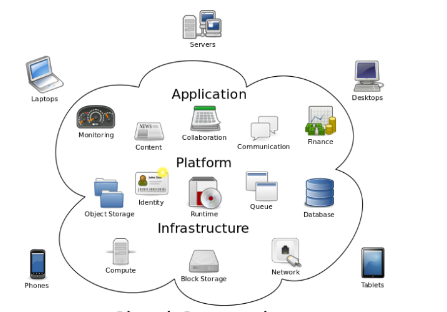
\includegraphics[scale=0.6]{figures/cloud_computing.png}
\caption{figure:cloudcomputing}
\label{fig1}
\end{center}
\section{L'�volution de Cloud computing:}
Le Cloud computing est le fruit d'une �volution technologique peuvent �tre pr�sent�e en 5 phases :
\begin{description}
 \item [*] Elle d�bute avec les Fournisseurs d'Acc�s Internet (FAI 1.0). Ils ont pour but de mettre en place des moyens de t�l�communication pour assurer le raccordement des personnes ou entreprises au r�seau internet.
 \item [*]La seconde phase est l'orientation des FAI vers l'h�bergement de pages web (FAI 2.0). Cette phase marque un grand bond dans le d�veloppement d'internet.
 \item [*] La troisi�me phase (FAI 3.0) est la possibilit� qu'offrent les FAI � h�berger des applications m�tiers des entreprises.
 \item [*] Une connaissance des besoins applicatifs des entreprises permettent aux FAI de faire �voluer leur domaine d'intervention. Ils mettent en place des plateformes de g�n�ration d'applications � la demande. Il s'agit des ASP (Application Service Provider) dont les "Software as a Service" sont des d�rives :c'est le FAI 4.0.
 \item [*] La g�n�ralisation des pratiques pr�c�dentes, la prise en compte de nouvelles pratiques et l'int�gration des principes que nous pr�sentons dans les sections suivantes donnent naissance au cloud computing \cite{Foster1999}.
 
\end{description}
\begin{center}
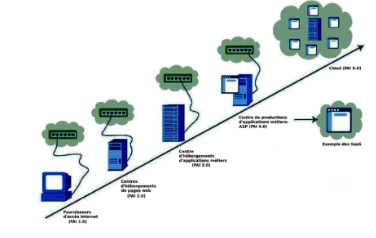
\includegraphics[scale=0.6]{figures/evolution_de_cloud_computing.png}

\caption{figure: evolution de cloud computing}
\label{fig2}
\end{center}
\section{Les caract�ristiques essentielles de cloud computing :}
\subsection{Self-service � la demande :}
L'utilisateur d'un service de � Cloud Computing � a la capacit� (� self-provisioning �)
d'approvisionner lui-m�me de nouvelles ressources telles que de l'espace disque, des serveurs virtuels, du temps CPU,m�moire vive RAM.
\subsection{Elasticit� et rapidit� :}
Les ressources peuvent �tre allou�es ou d�sallou�es rapidement. C'est une des caract�ristiques essentielles du Cloud computing , la capacit� d'augmenter et de r�duire le volume des ressources utilis�es en fonction des besoins, de m�me que lib�rer les ressources qui ne sont plus n�cessaires, au profit d'autres utilisations,Ces op�rations peuvent se faire par demande ou de fa�on automatique,par
programmation ou triggers.
\subsection{Acc�s aux ressources :}
Les ressources sont disponibles via le r�seau Internet, ou via l'Intranet dans le cas d'un Cloud priv�.
Les ressources sont accessibles via des protocoles standards (TCP/IP,SSL, HTTP,...)L'acc�s aux ressources peut se faire � partir d'un grand nombre de p�riph�riques clients (ordinateurs, portables, t�l�phones mobiles, smartphones, ...)et depuis n'importe quelle plate-forme (Windows, Unix, MacOs, Linux, syst�mes propri�taires,')
\subsection{Allocation des ressources :}
Les ressources mises � disposition par les providers de � Cloud Computing � sont mutualis�es pour r�pondre aux besoins de plusieurs clients dans une architecture multi-tenant. Une architecture � multi-tenant � ou � multi-locataire � fait qu'une seule instance d'une application est adapt�e aux besoins de tous les utilisateurs et offre malgr� tout un certain niveau de customisation pour s'adapter de mani�re individuel  aux diff�rents clients.
\subsection{Mesure du service :}
Toutes les ressources allou�es peuvent �tre surveill�es et contr�l�es de mani�re automatique ainsi que l'utilisation optimis�  de ressources  est assur�e en s'appuyant sur le mod�le ``payez uniquement ce que vous consommez''.
 \section{Taxonomie du cloud computing }
 Avant de pr�senter les diff�rents types de cloud pouvant �tre d�velopp�s, nous �tablissons dans un premier temps quelques crit�res de classification :
\begin{enumerate}
 \item {La raison de d�veloppement (business model):} c'est la raison qui justifie la mise en place de la plateforme. Elle peut �tre commerciale, scientifique ou communautaire...ex.
 \item {Le modele  de services :}c'est le modele de service que peut �tre d�livr� par le cloud aux clients.
 \item { L'accessibilit� :}Le cloud peut �tre accessible par tous (``cloud public'') ou restreint � un public particulier (``cloud priv�''), C'est la raison qui justifie le d�ploiement de la plateforme de cloud.
\end{enumerate}
\subsection{ raison de d�veloppement :}
L'utilisation du CC ne se limite pas uniquement aux entreprises � caract�re commercial. En fonction des raisons de sa mise en place, nous distinguons quatre cat�gories de plateformes de CC � savoir :
\begin{description}
 \item \textbf{Cloud d'Entreprises} :Dans cette cat�gorie, nous retrouvons des entreprises de petites et de moyennes tailles disposant chacune de peu de ressources et de moyens de maintenance de leurs infrastructures. Elles se regroupent donc autour d'un projet de cloud afin de mutualiser leurs capacit�s.La plateforme qui en d�coule est priv�e, c'est-a-dire accessible uniquement
par les entit�s des diff�rentes entreprises. Cette plateforme � l'avantage d'�tre de petite taille et d'acc�s restreint � des utilisateurs connus.
\item \textbf{Cloud Gouvernemental et Recherche Scientifique :}des instituts de recherche mettent leur pieds sur  des environnements de cloud pour des raison de recherche scientifique de developement ,L'acc�s est r�serv� aux personnes appartenant aux instituts de recherche associ�s.
\item \textbf{Cloud pour R�seaux Sociaux et Jeux :}Le d�veloppement des r�seaux sociaux et des jeux en ligne n�cessite de plus en plus de grandes quantit�s de ressources.ca implique la  d�veloppement d'une plateforme similaire au cloud devient une �vidence pour optimiser l'utilisation des ressources et faciliter le partage de donn�es. En effet, elles sont consid�r�es
comme un cloud .
\item \textbf{Cloud pour Fournisseurs de Services :}C'est le mod�le le plus r�pandu. Une entreprise, appel�e fournisseur, met � la disposition d'autres (appel�es clients) une plateforme d'ex�cution d'applications et assure le service informatique inh�rent.
\end{description}

\subsection{Le modele  de services:}
Le but principal du Cloud est d'offrir des services � des utilisateurs ,suivant diff�rents
mod�les.  NIST \cite{mell2011nist} pr�cise que le Cloud Computing a trois mod�les de services principaux Iaas,Paas,Saas
\begin{center}
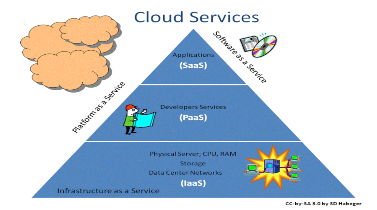
\includegraphics[scale=0.6]{figures/modele_de_service.png}

\caption{figure : modele de srvice}
\label{fig2}
\end{center}

\begin{description}
 \item \textbf{Infrastructure en tant que service(infrastructure as a Service  � Iaas �) :}
 Dans ce mod�le, l'infrastructure physique (le mat�riel r�seau, le mat�riel serveur, la plate-forme de
virtualisation, les moyens et capacit�s de stockage) est � d�mat�rialis�e � et h�berg�e.
Le fournisseur procure donc une couche mat�rielle (serveurs, r�seau, stockage, hyperviseur, solution de supervision, solution de management) sur laquelle les clients vont pouvoir d�poser leurs environnements syst�me et leurs applications.
Mais ce service va encore plus loin gr�ce � la virtualisation. L'utilisation de cette technologie permet aux clients de cr�er leur propre infrastructure personnalis�e (serveurs virtuels, r�seau virtuel, stockage) en quelques clicks. Cette infrastructure est par ailleurs extr�mement flexible, accessible sans restriction et configurable en temps r�el.
Les clients n'ont pas � se soucier de la scalabilit� de leur infrastructure, cette t�che �tant g�r�e par le fournisseur. Celui-ci g�re �galement tous les co�ts de gestion li�s au fonctionnement du mat�riel (�lectricit�, climatisation, etc) ainsi que le contr�le de la consommation s'il y a une facturation � l'usage (au Go, au temps d'utilisation, etc).
Il y a un avantage principal dans ce niveau de service. Le client n'a plus � construire son propre Datacenter, ni � g�rer l'infrastructure physique et les co�ts qui lui sont inh�rents.
L'ing�nieur ou l'administrateur syst�me peut se reconcentrer sur l'optimisation de son
environnement syst�me, et le d�veloppeur sur ses applications. En fait, le client � un contr�le total de son Datacenter virtuel sans se soucier de son �lasticit�, ni de l'infrastructurephysique qu'il y a derri�re.
Mais ce mod�le a �galement des inconv�nients. D�j�, comme pour toute infrastructure informatique classique, il est indispensable d'avoir un administrateur ou un ing�nieur syst�mes dans son entreprise. Et enfin, malgr� la facilit� technique de cr�ation d'une infrastructure personnalis�e gr�ce � la virtualisation, un important travail de r�flexion et d'expertise pr�alable reste � fournir pour sa mise en oeuvre.
Plusieurs offres existent dans cette cat�gorie comme Amazon Elastic Compute Cloud (EC2) ainsi que d'autre ElasticHosts, GoGrid, Rackspace Cloud,RightScale, Skytap et Orange Business.

\item \textbf{Plateforme en tant que service(Plateform as a Service � Paas �) :}Le PaaS fournit un niveau d'abstraction suppl�mentaire par rapport � l'IaaS. Dans cette cat�gorie, non seulement l'infrastructure est d�mat�rialis�e, mais aussi le syst�me d'exploitation, et la plateforme d'ex�cution, de d�ploiement et de d�veloppement'application.
Le fournisseur procure donc aux clients d�veloppeurs l'infrastructure, le syst�me d'exploitation, les bases de donn�es, la couche middleware, et une plateforme de d�veloppement compl�te, fonctionnelle et performante. Ces platesformes sont �quip�es d'outils de d�veloppement, de modules, d'un langage de programmation, d'un type de basede donn�es.
Le client d�veloppeur peut utiliser cette plate-forme pour h�berger, d�velopper et/ou ex�cuter des application.L'avantage pour le d�veloppeur est qu'il ne se soucie pas du mat�riel. Il peut d�velopper, d�ployer puis ex�cuter son application sans avoir � g�rer, ni les technologies sous-jacentes n�cessaires, ni les configurations mat�rielles.Le cycle de d�veloppement est fortement r�duit et le client peut de concentrer sur son application.
 L'inconv�nient apparait lorsque l'on veut d�placer une application d'une plateforme � une autre. La compatibilit� n'est pas av�r�e car en fonction des solutions les langages sont diff�rents. Il faut choisir sa plateforme en fonction de son langage, et ensuite y rester. 
\item \textbf{Logiciel en tant que service(Sofware as a Service � Saas �) :}
logiciel en tant que service (SaaS) offre des applications compl�tes fournies � la demande. Ce type de service fournit diff�rents types d'applications telle que webmail, suite de bureautique en ligne ainsi que les r�seaux sociaux et les jeux. Ces applications s'ex�cutent sur les infrastructures du provider. Elles sont h�berg�es sur le cloud et accessibles via un navigateur Internet. L'utilisation des services SaaS est plus simple que les autres services o� la facturation s'adapte dynamiquement avec la consommation et la param�trisation des services offerts sont limit�s. L'utilisateur n'a aucun souci sur l'installation des logiciels ou de leur mise � jour et il n'a aucun contr�le sur l'infrastructure du Cloud tel que serveurs virtuel, les composants r�seaux, l'emplacement de stockage, la version de
l'application et les fonctions d'application disponibles \cite{journals/computer/TurnerBB03}. On peut distinguer deux types principaux de logiciels ou applications en tant que services :
\begin{itemize}
 \item Des applications sont disponibles au publique g�n�ral totalement gratuit,par exemple Services Gmail et Facebook, o� les e-mails, pi�ces jointes des email, photos, vid�os et musiques. G�n�ralement ce type d'application est indirectement financ� par la publicit�, ou par des produits d�riv�s de l'analyse statistique � grande �chelle.
 \item des applications sont disponibles pour r�pondre aux attentes des entreprises payantes selon la consommation. Ces applications sont con�ues pour fournir des logiciels faciles � utiliser
\end{itemize}
\end{description}
\subsection{L'accessibilit� :}
En plus des mod�les de livraison qui permettent de concr�tiser les services Cloud, on trouve un ensemble de mod�les de d�ploiement de services bas�s Cloud computing. Ces mod�les permettent de d�finir le degr� d'acc�s de l'utilisateur final aux fournisseurs de services Cloud. Ces mod�les sont divis�s en quatre grandes cat�gories d'apr�s NIST\cite{mell2011nist}.
\begin{center}
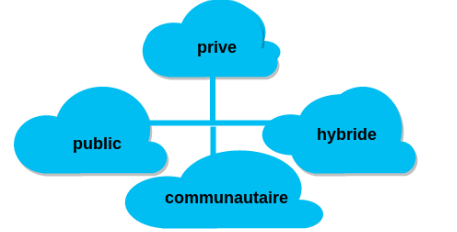
\includegraphics[scale=0.6]{figures/modele_de_deployement.png}

\caption{figure : modele de deployement}
\label{fig3}
\end{center}
\begin{description}
 \item \textbf{Le Cloud priv� :}
 Un cloud priv� est une infrastructure de cloud n'est utilis� que par une seule organisation. Le cloud priv� peut �tre g�r�e par l'organisation elle-m�me ou par un prestataire de service qui peut �tre situ�e dans les locaux de l'organisation ou � l'externe chez le prestataire de services. L'avantage suppl�mentaire du cloud priv� c'est  le contr�le total des donn�es par l'organisation, d'autre fa�on il permet la confidentialit� et la s�curit� des donn�es gr�ce aux ressources qui ne peuvent pas �tre partag�es par d'autres organisations \cite {conf/closer/ConwayC12}.
 \item \textbf{Le Cloud communautaire :}
L'architecture est d�di�e � une communaut� professionnelle sp�cifique, pour permettre de travailler de mani�re collaborative sur un m�me projet. 
 \item \textbf{Le Cloud public :}
Le cloud public est accessible publiquement � tous les particuliers et les groupes industriels. Son propri�taire est un fournisseur de service IaaS, PaaS ou SaaS. Les consommateurs ne sont factur�s que pour les applications, les services ou les donn�es qu'ils utilisent. Les ressources sont illimit�es et il n'y a donc aucun investissement initial. Les � Clouds � publics sont g�n�ralement exploit�s par des les fournisseurs de cloud commerciaux comme Amazon, Google, Microsoft, GoGrid.
 \item \textbf{Le Cloud hybride :}
Le cloud hybride est une composition de deux ou plusieurs infrastructures de Cloud publics et priv�s. G�n�ralement les donn�es sensibles sont g�r�es  au niveau interne par l'organisation ou chez le prestataire de cloud prive et l'autre type de donn�es � non-sensibles � sont g�r�es par le cloud publique
 \end{description}
\section{providers cloud computing }
l'existence du � cloud computing �et sa valeur pour les consommateurs sont aujourd'hui plus �videntes pour le grand public ,les diff�rents acteurs du monde IT comme Google et Microsoft proposent des services de Cloud Computing.
\begin{center}
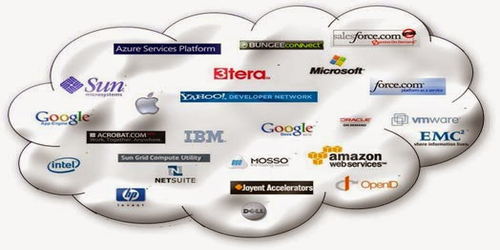
\includegraphics[scale=0.6]{figures/cloud_providers.png}

\caption{figure : cloud provider}
\label{fig4}
\end{center}
 \subsection{Amazon :}� Amazon Web Services � (AWS) met � disposition un cloud public depuis 2006. Au d�part le but d'Amazon �tait de rentabiliser ses �normes infrastructures requises pour assumer les
mont�es en charge pendant la p�riode de No�l sur leur boutique en ligne.
Aujourd'hui Amazon propose de nombreux services en ligne, � commencer par l'IaaS probablement le plus connu : Elastic Compute Cloud (EC2).
\subsection{Salesforce :}Salesforce.com est une soci�t� qui a lanc� d�s 2003 des offres de Cloud public. C'est officiellement le plus ancien prestataire dans ce domaine. Aujourd'hui encore, leurs offres sont uniquement compos�es de Cloud Public, et adress�es aux entreprises (surtout les grands comptes). Les outils propos�s sont tourn�s vers le travail collaboratif, la gestion des ventes et le marketing relationnel.
\subsection{Google AppEngine :}
Google mis et  propose beaucoup de services PaaS et SaaS sur le cloud computing . A grande �chelle, les solutions de Google dans le cloud sont surtout connues des consommateurs priv�s au travers des ses Google Apps telles que Google Docs, Calendar ou encore Gmail. Toutes ces � web apps � sont dans le domaine du SaaS et gratuites pour une utilisation priv�e. Google App Engine dont la premi�re version beta est sortie en avril 2008 est le service PaaS de Google. Au d�part le service ne supportait que le d�veloppement d'applications en Python. Depuis, le support de Java Virtual Machines (JVMs) a �t� ajout� et permet de d�velopper des applications non seulement en Java mais aussi au moyen de JRuby, JPython, Scala ou Clojure. Le SDK (software development kit) inclut un environnement complet de d�veloppement qui simule App Engine en local sur le bureau du d�veloppeur (Rhoton, 2010). La plateforme inclut �galement des services sous formes d'API permettant de manipuler des images, d'envoyer des mails ou encore d'utiliser les comptes Google pour les identifications au sein de l'application.
\subsection{Windows Azure :}
Microsoft s?av�re �tre actuellement l?un des seul acteur au niveau mondial � proposer des offres sur les trois mod�les SaaS, PaaS et IaaS. Les principales solutions SaaS sont Offices 365 et Microsoft Online Services. Windows Azure est le service PaaS phare de Microsoft. Avec la plateforme il est possible de migrer une application existante ou de d�velopper dans diff�rents langages de programmation, La plateforme met �galement � disposition le service SQL Azure, un service de base de donn�es bas�e sur Microsoft SQL Server. Au niveau IaaS, Microsoft propose une solution de cloud priv� qui repose sur Windows server.
\section{Conclusion : }
Le Cloud Computing se positionne actuellement en t�te de liste des nouvelles technologies. Il se caract�rise par son extensibilit� et �lasticit� et son exploitabilit� par un grand nombre d'utilisateurs dans le monde entier .il offre une grande puissance de calcul et espace de stockage, comme toute innovation technologique qui se respecte, le nuage informatique fait �conomiser de l'argent, le co�t, le temps d'utilisations des logiciels, leur d�veloppement et leur l'installation.



\chapter{D�ploiement d'applications}
\section{Introduction}
Le Cloud Computing se positionne actuellement en t�te de liste des nouvelles technologies. Il
se caract�rise par son extensibilit� et �lasticit� et son exploitabilit� par un grand nombre
d'utilisateurs dans le monde entier. 

Des nombreux individus et organisations ont choisi de d�placer leurs serveurs ou applications
dans un environnement en nuage afin d'optimiser l'utilisation de leur infrastructure informatique ,passage � l'�chelle, haute disponibilit�, etc.., L'exploitation des ressources d'infrastructure dans un environnement partag�,
ou mis en commun, permet de g�n�rer des �conomies de co�ts,le deplacement d'une application correspond au processus de red�ploiement de celle-ci, g�n�ralement sur de nouvelles plates-formes et au sein d'une nouvelle infrastructure. 

D'une mani�re g�n�rale, il existe deux mod�les de service cible potentiels pour la migration d'une application Infrastructure en tant que service (IaaS) et Platform as a Service (PaaS).
pour deployer un application chez les cloud provider il faut la bien configur�es et dimensionner l'environnement d'ex�cution,les d�pendances de l'application pour prendre en compte
l'h�t�rog�n�it� et l'�lasticit� inh�rentes au paradigme du Cloud Computing .

Notamment, il existe un grand nombre de provider ayant des niveaux de fonctionnalit� et des possibilit�s de dimensionnement h�t�rog�nes parmi les diff�rentes solutions de cloud disponibles (Amazon EC2, Rackspace cloud , WindowsAzure). Lors d'un d�ploiement d'application sur un PaaS, il faut choisir un
serveur d'application, la fr�quence CPU n�cessaire � l'ex�cution, la base de donn�es � utiliser, sa capacit� en terme espace m�moire, etc. Cette variabilit� en
termes de configuration et de dimensionnement offre une multitude de possibilit�s de configurations qui sont g�n�ralement effectu�es de mani�re ad hoc et sont
sources d'erreurs lorsqu'elles sont configur�es � la main\cite {quinton:hal-00747319}.



\section{D�finition du d�ploiement }
Apr�s avoir d�velopp� un application , vous  pouvez le d�ployer, nous pr�sentons trois grandes  d�finition  sur le d�ploiement : 
Nous commencerons par la d�finition de Clemens Szyperski \cite {conf/icse/Szyperski03},puis  nous poursuivrons par celle propos�e par l'Object
Management Group (OMG) \cite {web/omg} et enfin, nous finirons par la d�finition D�finition de Alan Dearle \cite {alan/Dearle07} .
.
\subsection{D�finition de C. Szyperski}
La d�finition du d�ploiement propos�e par C. Szyperski  c'est une d�finition g�n�rale du d�ploiement pour le domaine des composants logiciels, sans pour autant pr�ciser si elle se limite au d�ploiement sur le cloud computing  ou non. Le d�ploiement est d�fini comme �tant l'�tape de pr�paration d'un composant en vue de l'installer dans un environnement sp�cifique. C. Szyperski pr�cise explicitement que le d�ploiement (c'est-�-dire, la pr�paration) revient � renseigner les param�tres d'un descripteur de d�ploiement \cite {conf/icse/Szyperski03}. 
 
Nous pr�sentons les �tapes qui pr�c�dent et qui suivent cette phase de d�ploiement. 
Cela va nous permettre de pr�ciser ou cette phase de d�ploiement est situ�e dans le cycle de vie logiciel et quelle est sa port�e.
L'�tape qui pr�c�de le d�ploiement est l'acquisition. Cette �tape permet d'obtenir un composant logiciel. 
C. Szyperski �nonce que tout composant acquis est d�ployable. 
Ce qui signifie qu'un composant propos� � l'acquisition est produit ex�cutable par une machine physique ou virtuelle.
Plus pr�cis�ment, dans \cite {conf/icse/Szyperski03}, l'auteur met en avant le fait que tout composant doit �tre une unit� de d�ploiement (page 686).
Il d�finit ensuite une unit� de d�ploiement comme un d�livrable ex�cutable dans un environnement d'ex�cution, 
sans besoin d'intervention humaine pour modifier le composant afin de le rendre effectivement installable et pr�t � �tre ex�cut�. 
L'installation est l'�tape qui suit imm�diatement le d�ploiement. Elle rend un composant disponible sur un site (host) particulier,
dans un environnement particulier. Il est pr�cis� que cette �tape d'installation est souvent automatis�e. 
Enfin, l'�tape d'installation est suivie par le chargement (Loading) qui consiste � lancer l'ex�cution d'un composant dans un contexte d'ex�cution particulier.
\begin{center}
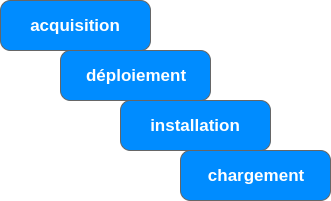
\includegraphics[scale=0.6]{figures/la_phase_de_deploiement.png}

\caption{figure :la phase de d�ploiement et son context selon Szyperski}
\label{fig5}
\end{center}
\subsection{D�finition de l'Object Management Group}
La phase de d�ploiement est constitue de cinq �tapes, � savoir, l'Installation, la Configuration, le Planning, la pr�paration et le Launch. Ces cinq �tapes sont structur�es les unes apr�s les autres de mani�re lin�aire et s�quentielle.  
 
La premi�re �tape est l'installation. Elle est d�finie comme la r�cup�ration, l'acquisition d'un package logiciel (software package) publi� et son rapatriement dans un d�p�t logiciel sous le contr�le du d�ployeur. Un d�p�t peut se situer, ou non, sur la m�me machine ou sur le m�me syst�me de fichier que celui dans lequel le logiciel va �tre d�ploy�. C'est une zone qui permet au d�ployeur d'appliquer des politiques au logiciel, comme l'authentification ou la certification (du logiciel), avant de lancer toute �tape concernant l'ex�cution du logiciel � proprement dit. Un d�p�t ne doit pas n�cessairement �tre persistant et ne doit pas, non plus, n�cessairement �tre stocker ou avoir une copie du logiciel ou des m�tadonn�es du logiciel. L'OMG propose, aussi, sa propre d�finition de l'activit� d'installation. Ainsi, l'installation n'est pas d�finie comme le d�placement d'un logiciel vers l'environnement d'ex�cution o� il pourra ensuite �tre activ�, mais simplement comme le d�placement du logiciel acquis vers le d�p�t du d�ployeur. 
 
La seconde �tape du processus de d�ploiement est la configuration. Pour r�aliser une configuration, un package logiciel doit �tre install� dans le d�p�t du d�ployeur. Le d�ployeur est le seul � pouvoir effectivement le configurer. Les possibilit�s de configuration offertes d�pendent de chaque package logiciel. Un package logiciel peut, par exemple, offrir des options de configuration concernant la langue � utiliser, le syst�me de mesure, le d�lai d'attente entre chaque mesure ou encore la fr�quence et le formatage des rapports de mesures g�n�r�s. Plusieurs configurations peuvent �tre associ�es � un m�me package logiciel. Enfin, cette seconde �tape ne concerne que la configuration des fonctions du package logiciel et n'est en aucun cas destin�e � la prise de d�cisions concernant le d�ploiement comme, par exemple, le choix de l'impl�mentation � utiliser ou, le cas �ch�ant, le choix de la distribution des diff�rents �l�ments du package logiciel. 
 
La troisi�me �tape s'articule sur la planification (Planning). Son but est de d�finir comment et ou une configuration va �tre ex�cut�e dans l'environnement cible. Pour rappel, la sp�cification d�finit un environnement comme �tant une infrastructure compos�e d'ordinateurs et de r�seaux. L'activit� de planification prend en compte les requis de la configuration � d�ployer, ainsi que les ressources offertes par l'environnement cible et s�lectionne les impl�mentations � utiliser. Elle d�cide �galement comment et o� la configuration donn�e sera ex�cut�e dans l'environnement cible. Le r�sultat de l'�tape de planification est un plan de d�ploiement sp�cifique (� la configuration en cours de d�ploiement, ainsi qu'� l'environnement cible). Le d�ploiement ainsi mis en  �uvre est un d�ploiement sensible au contexte. 
 
L'�tape avant derni�re �tape est nomm�e pr�paration. Elle est d�finie comme la mise en  �uvre effective des d�cisions prises lors de la planification. Ces d�cisions sont sp�cifi�es dans le plan de d�ploiement. Le but de la pr�paration est de rendre le logiciel pr�t � �tre ex�cut�. Cette mise en  ouvre consiste, entre autre, � d�placer des binaires ex�cutables dans les ordinateurs qui leur ont �t� attribu�s. Comme pour la planification deux modes de pr�paration sont distingu�s. Le premier est le mode juste � temps, le second est le mode par avance. Le mode juste � temps implique que l'�tape de pr�paration doit imm�diatement �tre suivie par l'�tape de lancement. Le mode par avance n'impose pas cette contrainte. 
La derni�re �tape est le lancement (Launch). Elle consiste � d�marrer l'ex�cution du logiciel, en collectant,  toutes les ressources  requises par le ou les packages logiciels dans l'environnement d'ex�cution. Afin de  lancer une application � base de composants ,il faut instancier des composants dans les ordinateurs de l'environnement cible, la configuration de ces instances de composants et la mise en place des interactions entre les diff�rentes instances et enfin, le d�marrage de l'ex�cution de l'application en elle-m�me.  
D�s que l'application s'ex�cute alors, soit l'application s'ex�cute malgr� que son ex�cution n'est pas compl�te, soit elle est arr�t�e (c'est-�-dire d�sactiv�e) en utilisant la m�me infrastructure de d�ploiement que celle par laquelle son lancement a �t� effectu� [lien vers le m�moire]. 
 
Les phases que nous venons de pr�senter peuvent tout � fait �tre d�roul�es une par une s�par�ment, ou comme une seule grande �tape de d�ploiement enti�rement automatis�e. 
 
\begin{center}
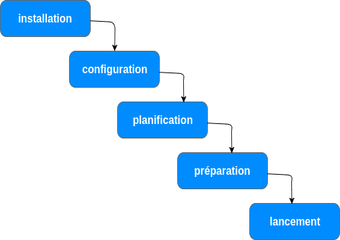
\includegraphics[scale=0.6]{figures/deploiement_omg.png}

\caption{figure :la phase de d�ploiement et son context selon OMG]}
\label{fig6}
\end{center}

\subsection{D�finition de Alan Dearle}
Le d�ploiement de logiciel est d�fini dans \cite {alan/Dearle07}comme le processus, constitu�
d?un ensemble d?activit�s li�es, entre l?acquisition et l?ex�cution du logiciel. Ce processus
a pour objectif de rendre op�rationnel une application, qui peut ainsi �tre utilis�e par
les utilisateurs. Une fois l?application d�ploy�e, le processus de d�ploiement continue
par les m�canismes d?adaptation du logiciel afin de chercher � atteindre une qualit� de
service. En effet, les infrastructures modernes sur lesquelles on d�ploie des applications
sont caract�ris�es par de fr�quentes variations de leur environnement.
Cependant, l?objectif d?un d�ploiement de logiciel, en plus de ceux d�j� not�s dans ces
d�finitions, peut �tre de maintenir une qualit� de service autre que la seule disponibilit�,
et que la non-atteinte de cette qualit�, provoque une strat�gie de red�ploiement. Cette
qualit� de service peut �tre qualitative (par exemple maintenir une topologie particuli�re)
ou bien quantitative (par exemple le logiciel devra �tre capable de r�aliser certaines t�ches
dans un temps inf�rieur � une valeur donn�e).
Ainsi, s?appuyant sur les d�finitions pr�c�dentes, on peut d�finir le d�ploiement de
logiciel comme un processus consistant en un ensemble d?activit�s reli�es et ayant pour
but de rendre le logiciel disponible � l?utilisation, � jour et en �tat d?assurer une qualit�
de service pr�d�finie.
Le processus de d�ploiement suppose au moins l?existence d?un logiciel qu?on veut
d�ployer, d?une infrastructure cible, constitu�e de ressources informatiques (ordinateurs,clusters, t�l�phones,...) interconnect�es, sur laquelle le logiciel sera d�ploy�, et, �ventuelle-
ment, d?outils permettant d?automatiser le d�ploiement (sinon l?op�ration sera effectu�e
manuellement)\cite {faye:tel-01280722}.

\section{Travaux connexes}
Nous  pr�sentons dans cette section les principaux approches de d�ploiement automatique  d'applications sur le cloud existent dans la litt�rature ,
ainsi nous citons les solutions les plus r�pondus actuellement
\subsection{Les approches de d�ploiement}
Il existe plusieurs solution �?outils et framworks � de d�ploiement automatique des logiciel dans
le cloud computing s'implique l'existence de plusieurs approche de base derri�re ces solutions. 
\subsubsection{Les scripts}
Pour faire face au d�ploiement automatique, diff�rents outils et solutions utilisent la codification manuelle par le biais de scripts,
ce qui n�cessite plus de temps pour d�ployer le logiciel.
Ce type d'approche r�duit le risque d'erreur humaine lors du processus de d�ploiement manuelle, et pour le cas de d�veloppeur, 
il s'occupe de d�veloppement d'application au lieu la configuration du cloud. Le seul inconv�nient de ces approches de d�ploiement,
c'est qu'il augmente les co�ts associ�s � la codification, le temps et les efforts humains \cite {ribeiro2016model}.

\subsubsection{Les approches semi-automatiques}
En outre, les mod�les virtuels propos�s par Disnix [Disnix] ont pr�sent� des m�canismes  
semi-automatis�s pour le d�ploiement. En d'autres termes, ces approches n�cessitent encore que certaines �tapes sont effectu�es manuellement pendant le processus de d�ploiement.
La solution propos�e par Ardagna [Ardagna ] a pr�sent� une approche partiellement orient�e et semi-automatis�e pour le d�ploiement de logiciel.
Elle exige un certain niveau de la compr�hension de l'utilisateur final sur les d�tails de la structure des clouds et une charge lourde de l'information dans les mod�les de d�ploiement demand� � l'utilisateur. 
\subsubsection{Les Workflow}
Cette solution propose que les d�veloppeurs aient les services � d�ployer pour cr�er les mod�les UML du d�ploiement de logiciels.
Ces mod�les d�finissent tous les informations requises pour le d�ploiement (machines virtuelles, services, applications, syst�mes d'exploitation des machines virtuelles,
des bases de donn�es, fournisseur de services et les cl�s d'acc�s) en tant que param�tres sans la n�cessit� du codage de la configuration d'une machine virtuelle.
Ces mod�les sont transform�s pour g�n�rer le code de d�ploiement � l'aide d'outils sp�cialis�s. 
le code de d�ploiement � l'aide d'outils sp�cialis�s.
\subsubsection{Approche bas�e sur les mod�les}
L'objectif est de d�ployer le logiciel � un niveau plus �lev� d'abstraction pour r�duire les efforts humains et le temps pass� � effectuer la t�che de d�ploiement, car l'approche bas�e sur un mod�le est une meilleure fa�on d'augmenter la productivit� de d�veloppeur.
Cette approche est la proposition de l'OMG qui est en cours de standardisation. 
La sp�cification de l'OMG, elle a pour objectif de fournir un mod�le de donn�es et d'ex�cution permettant de g�rer le d�veloppement, le packaging, le d�ploiement et la configuration d'applications � base de composants.
La sp�cification est d�crite � travers une entit� appel�e "Platform-Independent Model" (PIM), compos�e d'un ensemble de mod�les UML et de r�gles s�mantiques associ�es.
Le PIM est ind�pendant de tout mod�le de composant particulier. Pour utiliser cette sp�cification avec un mod�le particulier de composant, il faut cr�er une entit� appel�e "Platform-Specific Mapping" (PSM). Le PSM est un ensemble de r�gles qui transforme les mod�les UML du PIM en donn�es et mod�les d'ex�cution, dans un format appropri� pour le d�ploiement du mod�le de composant cible. La sp�cification n'a pour l'instant standardis� que le PSM pour le mod�le de composant Corba, dans lequel les mod�les de donn�es et d'ex�cution sont transform�s en deux formats : XML sch�ma pour le stockage sur disque et l'�change entre outils, 
et IDL (Interface Definition Language) pour la repr�sentation du mod�le d'ex�cution et des communications entre les entit�s du d�ploiement.
\section{Outils et frameworks de d�ploiement}
D'apr�s une �tude bibliographique sur les travaux qui s'articulent sur le d�ploiement 
automatique des logiciels sur le cloud computing, nous avons s�lectionn� les principaux outils 
et frameworks de d�ploiement afin de les d�crire :
\begin{enumerate}
\item L'outil SALOON est un outil de configuration et de d�ploiement. Bas� sur des ontologies, 
SALOON permet de sp�cifier une configuration technique pour l'application � d�ployer et de 
dimensionner cette configuration

\item La solution de Franklin est bas�e sur les mod�les pour le d�ploiement automatique des 
logiciels sur le cloud computing. Cette solution ne n�cessite que le d�veloppeur d'avoir des 
connaissances � propos de la cl� d'acc�s et le nom du fournisseur de services, �tant donn� que 
les d�tails sp�cifiques sont distraits. L'objectif est de d�ployer le logiciel � un niveau plus 
�lev� d'abstraction et r�duire les efforts humains et le temps pass� � effectuer pour le 
d�ploiement des t�ches, car l'approche bas�e sur les mod�les est une meilleure fa�on 
d'augmenter la productivit� du d�veloppeur\cite {moda} . 
 
 \item moSaIC Le projet europ�en de recherche mOSAIC \cite{conf/fedcsis/MoscatoAMFM11} propose une API et une plateformePaaS libre permettant de d�velopper et d�ployer des applications � ca n�cessite pas l?intervention directe du d�veloppeur d?application � pour un environnement multi-clouds. Ils se concentrent sur l?abstraction pour les d�veloppeurs d'applications et l'�tat peut facilement activer les utilisateurs pour "obtenir les caract�ristiques d'application souhait�es (comme l'�volutivit�, la tol�rance aux pannes,QoS ..etc.) "\cite{conf/servicewave/PetcuCNPMVRA10}. Il existe deux couches d'abstraction, une pour l'approvisionnement en cloud et une pour la logique d'application. La solution mOSAIC s�lectionnera un cloud appropri� sur la fa�on dont les d�veloppeurs d�crivent leur application, plusieurs providers cloud peuvent �tre s�lectionn�s en fonction de leurs propri�t�s.La construction d?une application d�ploy�e avec mOSAIC exige que cette derni�resoit constitu�e de composants avec des d�pendances explicites pour communiquer et�changer des donn�es entre eux. En outre, l?architecture de l?application doit �tre de type SOA et doit utiliser uniquement l?API mOSAIC pour la communication. mOSAIC utilise uniquement la communication asynchrone �technologies de files d'attente bas�es sur le cloud

\item Le projet europ�en de recherche RESERVOIR \cite{journals/ibmrd/RochwergerBLGNLMWECBEG09} vise � d�velopper une infrastructure de f�d�ration cloud entre les cloudspriv� et hybride afin de permettre  l?interop�rabilit� dynamique entre les fournisseurs de cloud. Avec cela, une application d�ploy�e peut r�partir la charge de travail de mani�re transparente entre les clouds priv�s et publics en fonction des exigences des applications. La transparence est r�alis�e en cr�ant des sites de r�servoir, un pour chaque fournisseur. Chaque site est ind�pendant et ex�cuteun environnement d'ex�cution virtuelle (VEE) qui est g�r� par un VirtualExecution Environment Manager (VEEM). L'VEEM communique avec d'autresVEEM et sont en mesure de faire une f�d�ration entre les clouds. Chaque site doit avoir des composants logiciels r�servoirs install�s, ce qui le rend autonome et autocontr�le .

\item Vega framework est un framework de d�ploiement destin� � des d�ploiements cloud complets sur des topologies multi-niveaux, elles suivent �galement une approche bas�e sur un mod�le. La description d'une topologie donn�e se fait en utilisant des fichiers XML (eXtensible Markup Language) avec ces fichiers, les d�veloppeurs peuvent r�pliquer une pile. Le XML contient des informations sur les instances, telles qu?ostype pour le syst�me d'exploitation et la description de l'image pour d�crire les propri�t�s d'une instance telle que la quantit� de m�moire . 
Ils permettent �galement que les petits scripts soient �crits directement dans le XML via un neoud Runoncescript qui peut faire une configuration suppl�mentaire sur une propagation neoud. Un gestionnaire de ressources surveille les ressources dans un syst�me, regroupant des instancesapr�s leurs attributs .



\end{enumerate}

\section{Conclusion : }
Dans ce chapitre, nous avons d�crit trois d�finition les plus utilis�es de d�ploiement automatique des applications sur le cloud computing , Afin de facilit� le choix de la technique de d�ploiement automatique approprie dans les prochains chapitres, nous avons montr� les approches d' adoption du Cloud computing par les d�veloppeurs de logiciels impl�ment�es par certain outils et Framworks. 
 
Un des aspects essentiels de manipulation des approches de d�ploiement consiste � automatis� le d�ploiement gr�ce � l'utilisation des workflows en impl�mentant ces m�thodes et ces outils, Ceci a donn� l'id�e de chapitre suivant. 
%\include{Chapitre}
%\include{Chapter4}
\chapter*{Conclusion g�n�rale}
\addcontentsline{toc}{chapter}{Conclusion g�n�rale} \mtcaddchapter
\markboth{Conclusion g�n�rale}{}
\vspace{4cm}

Ici la conclusion....

\end{spacing}

\nocite{*}
\bibliographystyle{plain}
\bibliography{Biblio}


%--------------------------------------%
%     ANNEXES                           
%------------------------------------------
%\chapter*{Annexes}
%\addcontentsline{toc}{chapter}{Annexes}
%%%%%%%%%%%%%%%%%%%%%%%%%%%%%%%%%%%%%%%%%%%%
%\begin{appendix}
%-------------------Annexe 1-------------------%
%\include{Annexe1}

%-------------------Annexe 2-------------------%
%\include{Annexe2}
%-------------------Annexe 3 -------------------%
%\include{Annexe3}	
%\end{appendix}
\end{document}
